%%%%%%%%%%%%%%%%%%%%%%%%%%%%%%%%%%%%%%%%%
% Jacobs Landscape Poster
% LaTeX Template
% Version 1.0 (29/03/13)
%
% Created by:
% Computational Physics and Biophysics Group, Jacobs University
% https://teamwork.jacobs-university.de:8443/confluence/display/CoPandBiG/LaTeX+Poster
% 
% Further modified by:
% Nathaniel Johnston (nathaniel@njohnston.ca)
%
% This template has been downloaded from:
% http://www.LaTeXTemplates.com
%
% License:
% CC BY-NC-SA 3.0 (http://creativecommons.org/licenses/by-nc-sa/3.0/)
%
%%%%%%%%%%%%%%%%%%%%%%%%%%%%%%%%%%%%%%%%%

%----------------------------------------------------------------------------------------
%	PACKAGES AND OTHER DOCUMENT CONFIGURATIONS
%----------------------------------------------------------------------------------------

\documentclass[final]{beamer}

\usepackage[scale=1.24]{beamerposter} % Use the beamerposter package for laying out the poster
\usepackage[utf8]{inputenc}

\usetheme{confposter} % Use the confposter theme supplied with this template

\setbeamercolor{block title}{fg=nred,bg=white} % Colors of the block titles
\setbeamercolor{block body}{fg=black,bg=white} % Colors of the body of blocks
\setbeamercolor{block alerted title}{fg=white,bg=dblue!30} % Colors of the highlighted block titles
\setbeamercolor{block alerted body}{fg=black,bg=dblue!10} % Colors of the body of highlighted blocks
% Many more colors are available for use in beamerthemeconfposter.sty

%-----------------------------------------------------------
% Define the column widths and overall poster size
% To set effective sepwid, onecolwid and twocolwid values, first choose how many columns you want and how much separation you want between columns
% In this template, the separation width chosen is 0.024 of the paper width and a 4-column layout
% onecolwid should therefore be (1-(# of columns+1)*sepwid)/# of columns e.g. (1-(4+1)*0.024)/4 = 0.22
% Set twocolwid to be (2*onecolwid)+sepwid = 0.464
% Set threecolwid to be (3*onecolwid)+2*sepwid = 0.708

\newlength{\sepwid}
\newlength{\onecolwid}
\newlength{\twocolwid}
\newlength{\threecolwid}
\setlength{\paperwidth}{48in} % A0 width: 46.8in
\setlength{\paperheight}{36in} % A0 height: 33.1in
\setlength{\sepwid}{0.024\paperwidth} % Separation width (white space) between columns
\setlength{\onecolwid}{0.22\paperwidth} % Width of one column
\setlength{\twocolwid}{0.464\paperwidth} % Width of two columns
\setlength{\threecolwid}{0.708\paperwidth} % Width of three columns
\setlength{\topmargin}{-0.5in} % Reduce the top margin size
%-----------------------------------------------------------
\renewcommand{\figurename}{Fig.}

\definecolor{dorado}{RGB}{255,204,102}

\usepackage{graphicx}  % Required for including images

\usepackage{booktabs} % Top and bottom rules for tables

%----------------------------------------------------------------------------------------
%	TITLE SECTION 
%----------------------------------------------------------------------------------------

\title{Titolo della Lezione - Le Derivate \#01} % Poster title

\author{prof. Diego Fantinelli} % Author(s)

\institute{Liceo Scientifico "Jacopo Da Ponte" - Bassano del Grappa\\ {\em Dipartimento di Matematica}} % Institution(s)

%----------------------------------------------------------------------------------------

\begin{document}

\addtobeamertemplate{block end}{}{\vspace*{2ex}} % White space under blocks
\addtobeamertemplate{block alerted end}{}{\vspace*{2ex}} % White space under highlighted (alert) blocks

\setlength{\belowcaptionskip}{2ex} % White space under figures
\setlength\belowdisplayshortskip{2ex} % White space under equations

\begin{frame}[t] % The whole poster is enclosed in one beamer frame

\begin{columns}[t] % The whole poster consists of three major columns, the second of which is split into two columns twice - the [t] option aligns each column's content to the top

\begin{column}{\sepwid}\end{column} % Empty spacer column

\begin{column}{\onecolwid} % The first column

%----------------------------------------------------------------------------------------
%	OBJECTIVES
%----------------------------------------------------------------------------------------

\begin{block}{Obiettivi}
Este documento es un \emph{entrenamiento dirigido} lo que significa que esta redactado a manera de monólogo, pero con indicaciones para el lector. 
Se sugiere separar entre 10 y 20 minutos a su lectura y tener a la mano hojas blancas, material para escribir y juego de geometría.
Al final trata de encontrar a alguien para discutir las ideas que hayas tenido y especialmente para comentar las tuyas.
\end{block}

\begin{block}{Obiettivi}
El objetivo no es simplemente resolver los problemas, sino utilizarlos para desarrollar nuestras habilidades de razonamiento.
No pienses que "acabaste" solo porque encontraste la respuesta. Cada problema es una oportunidad de aprendizaje y es necesario que entiendas los puntos de vista de otras personas y sus formas de razonar. Esta es la única forma que conozco de desarrollar las habilidades de razonamiento.
\end{block}

%----------------------------------------------------------------------------------------
%	INTRODUCTION
%----------------------------------------------------------------------------------------

\begin{block}{Introduzione}
Lo más apasionante de las olimpiadas de matemáticas es que los acertijos no requieren saber muchas cosas. Es más importante la imaginación y las estrategias intelectuales de razonamiento.

Empecemos con un problema de geometría tomado del libro \cite{Posamentier:CPIG}. Dedica al menos 5 minutos a tratar de resolver este problema por tu propia cuenta sin consultar ninguna fuente de información externa.

\end{block}

\begin{alertblock}{Ricordando che\dots}
Imagina un triángulo $ABC$ y dos puntos $D, E$ en los lados $BC, AC$ respectivamente.
Las bisectrices internas de los ángulos $\angle DAC$ y $\angle CBE$ se cortan en el punto $F$.
Demuestra que la medida de $\angle AFB$ es el promedio de las medidas de $\angle AEB$ y $\angle ADB$.
\end{alertblock}

\end{column} % End of the first column

\begin{column}{\sepwid}\end{column} % Empty spacer column

\begin{column}{\onecolwid} % Begin a column which is two columns wide (column 2)

%\begin{columns}[t,totalwidth=\twocolwid] % Split up the two columns wide column

%\begin{column}{\onecolwid}\vspace{-.6in} % The first column within column 2 (column 2.1)

\begin{block}{Il problema}
Para este problema suponemos que conoces los conceptos de triángulo y ángulos. El único concepto con el que puedes tener dificultades es el de "bisectriz interna". 

Un \emph{ángulo} es la figura geométrica formada por dos semirrectas que tienen un vértice común. Se le llama \emph{bisectriz interna} al lugar geométrico de los puntos que están a la misma distancia de ambas semirrectas. En la figura siguiente las semirrectas que forman el ángulo están de color negro, el vértice está marcado y la recta roja indica la bisectriz interna. Aprovechamos el espacio para marcar una recta azul perpendicular a la bisectriz interna a la cual se le llama \emph{bisectriz externa}.


\end{block}
%------------------------------------------------


\begin{figure}
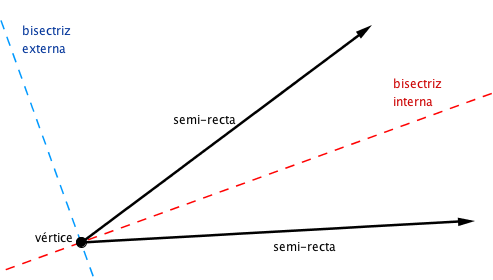
\includegraphics[width=0.8\linewidth]{bisectriz.png}
\caption{Bisectrices de un ángulo}
\end{figure}

\begin{block}{Graficamente}
En problemas de geometría, el entendimiento se demuestra trazando una figura clara que refleje toda la información del problema.
El diagrama siguiente presenta todo lo que dice el problema incluyendo la definición de variables para los ángulos involucrados. Quisiera hacer notar algunas sugerencias generales.

\begin{enumerate}
\item Explora diferentes configuraciones y evita los puntos o rectas empalmadas.
\item Usa el mínimo de variables que sea posible.
\item La información de bisectrices se refleja mejor con variables.  
\item No traces nada que no esté en el problema hasta que sea necesario hacerlo.
\end{enumerate}


\end{block}


\end{column} % End of column 2

\begin{column}{\onecolwid} 

\begin{figure}
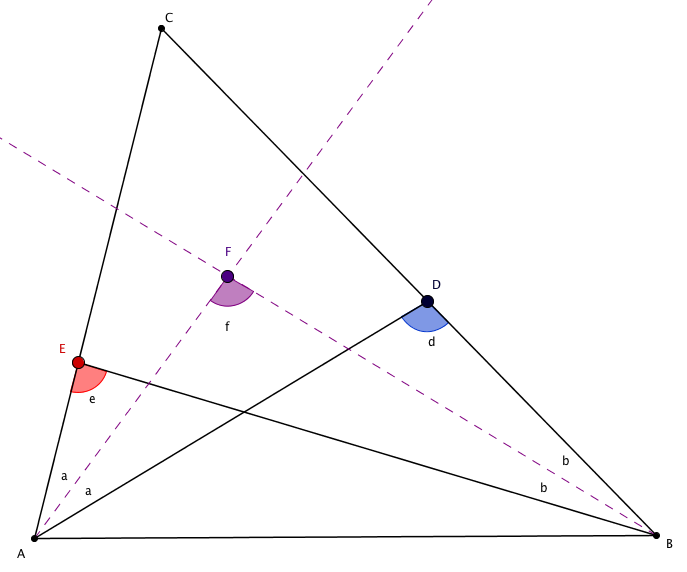
\includegraphics[width=0.8\linewidth]{CPIG_0101.png}
\caption{Diagrama del problema}
\end{figure}

\begin{block}{Osservazioni}
La parte creativa en la solución de problemas es el análisis de la situación. En este caso procuramos detectar patrones basados en nuestra experiencia previa.
En este problema los patrones deben estar relacionados con ángulos y triángulos. 

Un patrón que puedes usar es el conocido resultado de que la suma de los ángulos de un triángulo es $180^o$. Con esta idea puede resolverse el problema aunque tendrás que definir algunas variables adicionales. 

Un patrón que de hecho usa mejor la información es el siguiente que involucra dos triángulos que comparten un ángulo en común.
\begin{figure}
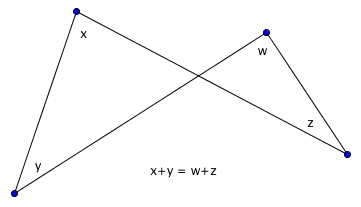
\includegraphics[width=0.8\linewidth]{mini_mariposa.png}
\caption{Triángulos con ángulo común}
\end{figure}

La experiencia en solución de problemas se adquiere mediante el dominio de patrones como este. Aunque estos pueden deducirse de resultados básicos, el no conocerlos puede significar la diferencia entre tener o no la idea correcta en problemas complejos.
\end{block}

\end{column} % End of column 3

\begin{column}{\sepwid}\end{column} % Empty spacer column

\begin{column}{\onecolwid} % The third column

%----------------------------------------------------------------------------------------
%	CONCLUSION
%----------------------------------------------------------------------------------------

\begin{block}{Esercizi}
Para que practiques te dejamos la siguiente lista de problemas relacionados con bisectrices.
\begin{enumerate}
\item Completa la demostración del problema usando dos veces el patrón de la figura 3.
\item Completa la demostración del problema de muestra usando solo que la suma de los ángulos de un triángulo es $180^o$
\item Analiza como se modifica el problema de muestra si los puntos $D, E$ están en las rectas $BC, AC$ pero fuera de los segmentos.
\item La bisectriz interna de $\angle B$ y la bisectriz externa de $\angle C$ de otro $\triangle ABC$ se cortan en $C$. Por $C$ se traza una paralela a $BC$ que corta $AC, AB$ en $L, M$. Si sabemos que $LC=5$ y $MB=7$, calcula la medida de $LM$.
\item En la hipotenusa $AB$ de un triángulo rectángulo $ABC$ se consideran puntos $D, E, F$ de modo que $CD \perp AB$, $CE$ es bisectriz interna de $\angle BCA$ y $F$ es punto medio de $AB$. Demuestra que $CE$ también es bisectriz de $\angle DCF$.
\item El segmento $PC$ es perpendicular a la hipotenusa $AC$ de un triángulo rectángulo $ABC$. Demuestra que $BP$ es perpendicular o paralelo a la bisectriz de $\angle BAC$.
\end{enumerate}
\end{block}

\begin{block}{Riferimenti}

\nocite{*} % Insert publications even if they are not cited in the poster
\small{\bibliographystyle{unsrt}
\bibliography{sample}\vspace{0.75in}}

\end{block}

\setbeamercolor{block alerted title}{fg=black,bg=dorado} % Change the alert block title colors
\setbeamercolor{block alerted body}{fg=black,bg=white} % Change the alert block body colors

\begin{alertblock}{Contatti}
Olimpiadas de Matemáticas en Nuevo León
\begin{itemize}
\item Web:
\href{http://olmatnl.blogspot.mx/}{http://olmatnl.blogspot.mx/}
\item Facebook: \href{https://www.facebook.com/olmatnl}{https://www.facebook.com/olmatnl}
\item Email: \href{mailto:}{diego.fantinelli@gmail.com}
\end{itemize}
\end{alertblock}

%----------------------------------------------------------------------------------------

\end{column} % End of the third column

\end{columns} % End of all the columns in the poster

\end{frame} % End of the enclosing frame

\end{document}
